% Created by tikzDevice version 0.6.2-92-0ad2792 on 2013-03-12 19:39:57
% !TEX encoding = UTF-8 Unicode
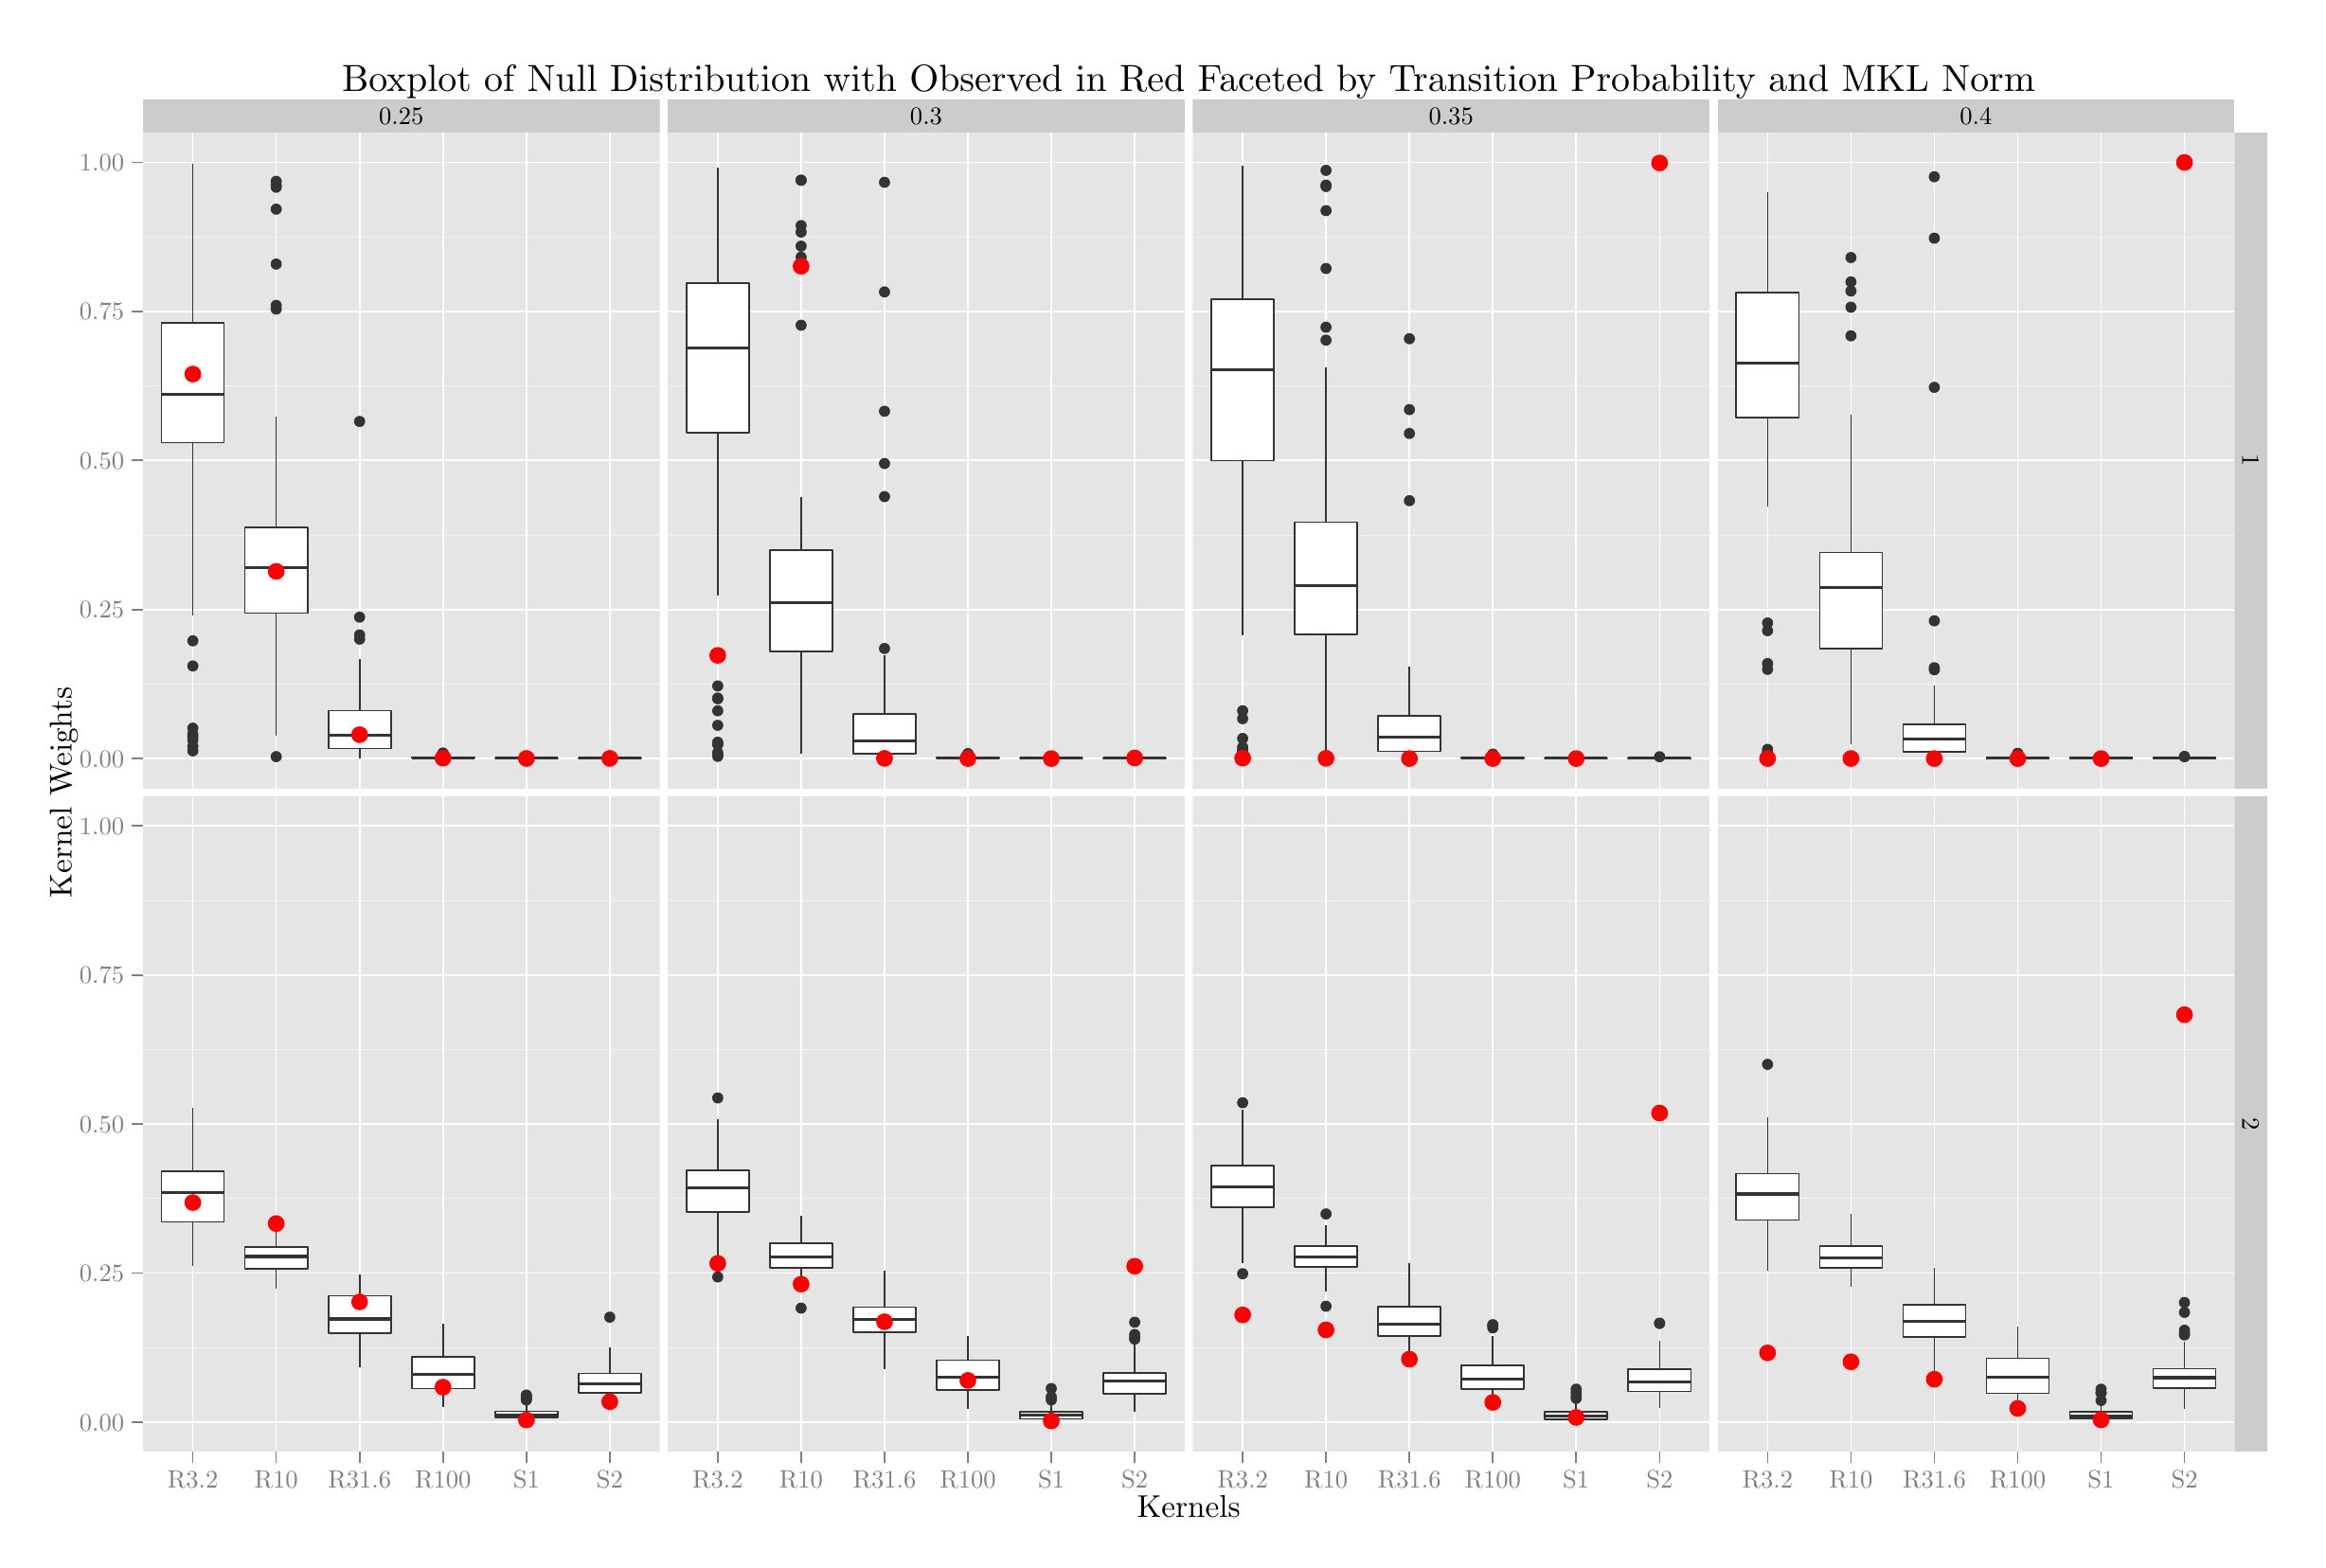
\begin{tikzpicture}[x=1pt,y=1pt]
\definecolor[named]{fillColor}{rgb}{1.00,1.00,1.00}
\path[use as bounding box,fill=fillColor,fill opacity=0.00] (0,0) rectangle (867.24,578.16);
\begin{scope}
\path[clip] (  0.00,  0.00) rectangle (867.24,578.16);
\definecolor[named]{drawColor}{rgb}{1.00,1.00,1.00}
\definecolor[named]{fillColor}{rgb}{1.00,1.00,1.00}

\path[draw=drawColor,line width= 0.6pt,line join=round,line cap=round,fill=fillColor] ( -0.00,  0.00) rectangle (867.24,578.16);
\end{scope}
\begin{scope}
\path[clip] ( 44.49,537.54) rectangle (241.75,550.17);
\definecolor[named]{fillColor}{rgb}{0.80,0.80,0.80}

\path[fill=fillColor] ( 44.49,537.54) rectangle (241.75,550.17);
\definecolor[named]{drawColor}{rgb}{0.00,0.00,0.00}

\node[text=drawColor,anchor=base,inner sep=0pt, outer sep=0pt, scale=  0.96] at (143.12,540.55) {0.25};
\end{scope}
\begin{scope}
\path[clip] (244.76,537.54) rectangle (442.02,550.17);
\definecolor[named]{fillColor}{rgb}{0.80,0.80,0.80}

\path[fill=fillColor] (244.76,537.54) rectangle (442.02,550.17);
\definecolor[named]{drawColor}{rgb}{0.00,0.00,0.00}

\node[text=drawColor,anchor=base,inner sep=0pt, outer sep=0pt, scale=  0.96] at (343.39,540.55) {0.3};
\end{scope}
\begin{scope}
\path[clip] (445.03,537.54) rectangle (642.29,550.17);
\definecolor[named]{fillColor}{rgb}{0.80,0.80,0.80}

\path[fill=fillColor] (445.03,537.54) rectangle (642.29,550.17);
\definecolor[named]{drawColor}{rgb}{0.00,0.00,0.00}

\node[text=drawColor,anchor=base,inner sep=0pt, outer sep=0pt, scale=  0.96] at (543.66,540.55) {0.35};
\end{scope}
\begin{scope}
\path[clip] (645.30,537.54) rectangle (842.56,550.17);
\definecolor[named]{fillColor}{rgb}{0.80,0.80,0.80}

\path[fill=fillColor] (645.30,537.54) rectangle (842.56,550.17);
\definecolor[named]{drawColor}{rgb}{0.00,0.00,0.00}

\node[text=drawColor,anchor=base,inner sep=0pt, outer sep=0pt, scale=  0.96] at (743.93,540.55) {0.4};
\end{scope}
\begin{scope}
\path[clip] ( 44.49,287.29) rectangle (241.75,537.54);
\definecolor[named]{fillColor}{rgb}{0.90,0.90,0.90}

\path[fill=fillColor] ( 44.49,287.29) rectangle (241.75,537.54);
\definecolor[named]{drawColor}{rgb}{0.95,0.95,0.95}

\path[draw=drawColor,line width= 0.3pt,line join=round] ( 44.49,327.11) --
	(241.75,327.11);

\path[draw=drawColor,line width= 0.3pt,line join=round] ( 44.49,384.01) --
	(241.75,384.01);

\path[draw=drawColor,line width= 0.3pt,line join=round] ( 44.49,440.90) --
	(241.75,440.90);

\path[draw=drawColor,line width= 0.3pt,line join=round] ( 44.49,497.79) --
	(241.75,497.79);
\definecolor[named]{drawColor}{rgb}{1.00,1.00,1.00}

\path[draw=drawColor,line width= 0.6pt,line join=round] ( 44.49,298.67) --
	(241.75,298.67);

\path[draw=drawColor,line width= 0.6pt,line join=round] ( 44.49,355.56) --
	(241.75,355.56);

\path[draw=drawColor,line width= 0.6pt,line join=round] ( 44.49,412.45) --
	(241.75,412.45);

\path[draw=drawColor,line width= 0.6pt,line join=round] ( 44.49,469.34) --
	(241.75,469.34);

\path[draw=drawColor,line width= 0.6pt,line join=round] ( 44.49,526.23) --
	(241.75,526.23);

\path[draw=drawColor,line width= 0.6pt,line join=round] ( 63.58,287.29) --
	( 63.58,537.54);

\path[draw=drawColor,line width= 0.6pt,line join=round] ( 95.39,287.29) --
	( 95.39,537.54);

\path[draw=drawColor,line width= 0.6pt,line join=round] (127.21,287.29) --
	(127.21,537.54);

\path[draw=drawColor,line width= 0.6pt,line join=round] (159.02,287.29) --
	(159.02,537.54);

\path[draw=drawColor,line width= 0.6pt,line join=round] (190.84,287.29) --
	(190.84,537.54);

\path[draw=drawColor,line width= 0.6pt,line join=round] (222.66,287.29) --
	(222.66,537.54);
\definecolor[named]{fillColor}{rgb}{0.20,0.20,0.20}

\path[fill=fillColor] ( 63.58,310.26) circle (  2.13);

\path[fill=fillColor] ( 63.58,334.01) circle (  2.13);

\path[fill=fillColor] ( 63.58,307.02) circle (  2.13);

\path[fill=fillColor] ( 63.58,301.60) circle (  2.13);

\path[fill=fillColor] ( 63.58,305.78) circle (  2.13);

\path[fill=fillColor] ( 63.58,343.59) circle (  2.13);

\path[fill=fillColor] ( 63.58,303.38) circle (  2.13);

\path[fill=fillColor] ( 63.58,307.96) circle (  2.13);
\definecolor[named]{drawColor}{rgb}{0.20,0.20,0.20}

\path[draw=drawColor,line width= 0.6pt,line join=round,fill=fillColor] ( 63.58,464.83) -- ( 63.58,525.48);

\path[draw=drawColor,line width= 0.6pt,line join=round,fill=fillColor] ( 63.58,419.18) -- ( 63.58,353.14);
\definecolor[named]{fillColor}{rgb}{1.00,1.00,1.00}

\path[draw=drawColor,line width= 0.6pt,line join=round,line cap=round,fill=fillColor] ( 51.64,464.83) --
	( 51.64,419.18) --
	( 75.51,419.18) --
	( 75.51,464.83) --
	( 51.64,464.83) --
	cycle;
\definecolor[named]{fillColor}{rgb}{0.20,0.20,0.20}

\path[draw=drawColor,line width= 1.1pt,line join=round,fill=fillColor] ( 51.64,437.63) -- ( 75.51,437.63);

\path[fill=fillColor] ( 95.39,299.40) circle (  2.13);

\path[fill=fillColor] ( 95.39,508.33) circle (  2.13);

\path[fill=fillColor] ( 95.39,470.20) circle (  2.13);

\path[fill=fillColor] ( 95.39,517.48) circle (  2.13);

\path[fill=fillColor] ( 95.39,518.95) circle (  2.13);

\path[fill=fillColor] ( 95.39,471.61) circle (  2.13);

\path[fill=fillColor] ( 95.39,487.37) circle (  2.13);

\path[fill=fillColor] ( 95.39,516.69) circle (  2.13);

\path[draw=drawColor,line width= 0.6pt,line join=round,fill=fillColor] ( 95.39,386.97) -- ( 95.39,429.30);

\path[draw=drawColor,line width= 0.6pt,line join=round,fill=fillColor] ( 95.39,354.16) -- ( 95.39,307.38);
\definecolor[named]{fillColor}{rgb}{1.00,1.00,1.00}

\path[draw=drawColor,line width= 0.6pt,line join=round,line cap=round,fill=fillColor] ( 83.46,386.97) --
	( 83.46,354.16) --
	(107.32,354.16) --
	(107.32,386.97) --
	( 83.46,386.97) --
	cycle;
\definecolor[named]{fillColor}{rgb}{0.20,0.20,0.20}

\path[draw=drawColor,line width= 1.1pt,line join=round,fill=fillColor] ( 83.46,371.44) -- (107.32,371.44);

\path[fill=fillColor] (127.21,345.84) circle (  2.13);

\path[fill=fillColor] (127.21,427.32) circle (  2.13);

\path[fill=fillColor] (127.21,344.24) circle (  2.13);

\path[fill=fillColor] (127.21,352.62) circle (  2.13);

\path[draw=drawColor,line width= 0.6pt,line join=round,fill=fillColor] (127.21,316.93) -- (127.21,336.58);

\path[draw=drawColor,line width= 0.6pt,line join=round,fill=fillColor] (127.21,302.49) -- (127.21,298.68);
\definecolor[named]{fillColor}{rgb}{1.00,1.00,1.00}

\path[draw=drawColor,line width= 0.6pt,line join=round,line cap=round,fill=fillColor] (115.28,316.93) --
	(115.28,302.49) --
	(139.14,302.49) --
	(139.14,316.93) --
	(115.28,316.93) --
	cycle;
\definecolor[named]{fillColor}{rgb}{0.20,0.20,0.20}

\path[draw=drawColor,line width= 1.1pt,line join=round,fill=fillColor] (115.28,307.62) -- (139.14,307.62);

\path[fill=fillColor] (159.02,299.75) circle (  2.13);

\path[fill=fillColor] (159.02,300.55) circle (  2.13);

\path[fill=fillColor] (159.02,299.78) circle (  2.13);

\path[fill=fillColor] (159.02,300.25) circle (  2.13);

\path[fill=fillColor] (159.02,300.04) circle (  2.13);

\path[fill=fillColor] (159.02,300.66) circle (  2.13);

\path[fill=fillColor] (159.02,300.33) circle (  2.13);

\path[fill=fillColor] (159.02,299.80) circle (  2.13);

\path[fill=fillColor] (159.02,300.77) circle (  2.13);

\path[fill=fillColor] (159.02,299.85) circle (  2.13);

\path[draw=drawColor,line width= 0.6pt,line join=round,fill=fillColor] (159.02,299.20) -- (159.02,299.74);

\path[draw=drawColor,line width= 0.6pt,line join=round,fill=fillColor] (159.02,298.84) -- (159.02,298.67);
\definecolor[named]{fillColor}{rgb}{1.00,1.00,1.00}

\path[draw=drawColor,line width= 0.6pt,line join=round,line cap=round,fill=fillColor] (147.09,299.20) --
	(147.09,298.84) --
	(170.95,298.84) --
	(170.95,299.20) --
	(147.09,299.20) --
	cycle;
\definecolor[named]{fillColor}{rgb}{0.20,0.20,0.20}

\path[draw=drawColor,line width= 1.1pt,line join=round,fill=fillColor] (147.09,298.99) -- (170.95,298.99);

\path[fill=fillColor] (190.84,299.11) circle (  2.13);

\path[draw=drawColor,line width= 0.6pt,line join=round,fill=fillColor] (190.84,298.81) -- (190.84,298.95);

\path[draw=drawColor,line width= 0.6pt,line join=round,fill=fillColor] (190.84,298.69) -- (190.84,298.67);
\definecolor[named]{fillColor}{rgb}{1.00,1.00,1.00}

\path[draw=drawColor,line width= 0.6pt,line join=round,line cap=round,fill=fillColor] (178.91,298.81) --
	(178.91,298.69) --
	(202.77,298.69) --
	(202.77,298.81) --
	(178.91,298.81) --
	cycle;
\definecolor[named]{fillColor}{rgb}{0.20,0.20,0.20}

\path[draw=drawColor,line width= 1.1pt,line join=round,fill=fillColor] (178.91,298.74) -- (202.77,298.74);

\path[fill=fillColor] (222.66,299.16) circle (  2.13);

\path[fill=fillColor] (222.66,299.27) circle (  2.13);

\path[fill=fillColor] (222.66,299.22) circle (  2.13);

\path[fill=fillColor] (222.66,299.30) circle (  2.13);

\path[fill=fillColor] (222.66,299.47) circle (  2.13);

\path[fill=fillColor] (222.66,299.33) circle (  2.13);

\path[draw=drawColor,line width= 0.6pt,line join=round,fill=fillColor] (222.66,298.88) -- (222.66,299.04);

\path[draw=drawColor,line width= 0.6pt,line join=round,fill=fillColor] (222.66,298.72) -- (222.66,298.67);
\definecolor[named]{fillColor}{rgb}{1.00,1.00,1.00}

\path[draw=drawColor,line width= 0.6pt,line join=round,line cap=round,fill=fillColor] (210.73,298.88) --
	(210.73,298.72) --
	(234.59,298.72) --
	(234.59,298.88) --
	(210.73,298.88) --
	cycle;
\definecolor[named]{fillColor}{rgb}{0.20,0.20,0.20}

\path[draw=drawColor,line width= 1.1pt,line join=round,fill=fillColor] (210.73,298.79) -- (234.59,298.79);
\definecolor[named]{fillColor}{rgb}{1.00,0.00,0.00}

\path[fill=fillColor] ( 63.58,445.40) circle (  3.20);

\path[fill=fillColor] ( 95.39,370.09) circle (  3.20);

\path[fill=fillColor] (127.21,307.78) circle (  3.20);

\path[fill=fillColor] (159.02,298.84) circle (  3.20);

\path[fill=fillColor] (190.84,298.71) circle (  3.20);

\path[fill=fillColor] (222.66,298.74) circle (  3.20);
\end{scope}
\begin{scope}
\path[clip] ( 44.49, 34.03) rectangle (241.75,284.28);
\definecolor[named]{fillColor}{rgb}{0.90,0.90,0.90}

\path[fill=fillColor] ( 44.49, 34.03) rectangle (241.75,284.28);
\definecolor[named]{drawColor}{rgb}{0.95,0.95,0.95}

\path[draw=drawColor,line width= 0.3pt,line join=round] ( 44.49, 73.85) --
	(241.75, 73.85);

\path[draw=drawColor,line width= 0.3pt,line join=round] ( 44.49,130.75) --
	(241.75,130.75);

\path[draw=drawColor,line width= 0.3pt,line join=round] ( 44.49,187.64) --
	(241.75,187.64);

\path[draw=drawColor,line width= 0.3pt,line join=round] ( 44.49,244.53) --
	(241.75,244.53);
\definecolor[named]{drawColor}{rgb}{1.00,1.00,1.00}

\path[draw=drawColor,line width= 0.6pt,line join=round] ( 44.49, 45.41) --
	(241.75, 45.41);

\path[draw=drawColor,line width= 0.6pt,line join=round] ( 44.49,102.30) --
	(241.75,102.30);

\path[draw=drawColor,line width= 0.6pt,line join=round] ( 44.49,159.19) --
	(241.75,159.19);

\path[draw=drawColor,line width= 0.6pt,line join=round] ( 44.49,216.08) --
	(241.75,216.08);

\path[draw=drawColor,line width= 0.6pt,line join=round] ( 44.49,272.98) --
	(241.75,272.98);

\path[draw=drawColor,line width= 0.6pt,line join=round] ( 63.58, 34.03) --
	( 63.58,284.28);

\path[draw=drawColor,line width= 0.6pt,line join=round] ( 95.39, 34.03) --
	( 95.39,284.28);

\path[draw=drawColor,line width= 0.6pt,line join=round] (127.21, 34.03) --
	(127.21,284.28);

\path[draw=drawColor,line width= 0.6pt,line join=round] (159.02, 34.03) --
	(159.02,284.28);

\path[draw=drawColor,line width= 0.6pt,line join=round] (190.84, 34.03) --
	(190.84,284.28);

\path[draw=drawColor,line width= 0.6pt,line join=round] (222.66, 34.03) --
	(222.66,284.28);
\definecolor[named]{drawColor}{rgb}{0.20,0.20,0.20}
\definecolor[named]{fillColor}{rgb}{0.20,0.20,0.20}

\path[draw=drawColor,line width= 0.6pt,line join=round,fill=fillColor] ( 63.58,141.23) -- ( 63.58,165.55);

\path[draw=drawColor,line width= 0.6pt,line join=round,fill=fillColor] ( 63.58,121.85) -- ( 63.58,104.90);
\definecolor[named]{fillColor}{rgb}{1.00,1.00,1.00}

\path[draw=drawColor,line width= 0.6pt,line join=round,line cap=round,fill=fillColor] ( 51.64,141.23) --
	( 51.64,121.85) --
	( 75.51,121.85) --
	( 75.51,141.23) --
	( 51.64,141.23) --
	cycle;
\definecolor[named]{fillColor}{rgb}{0.20,0.20,0.20}

\path[draw=drawColor,line width= 1.1pt,line join=round,fill=fillColor] ( 51.64,132.95) -- ( 75.51,132.95);

\path[draw=drawColor,line width= 0.6pt,line join=round,fill=fillColor] ( 95.39,112.37) -- ( 95.39,122.83);

\path[draw=drawColor,line width= 0.6pt,line join=round,fill=fillColor] ( 95.39,103.85) -- ( 95.39, 96.43);
\definecolor[named]{fillColor}{rgb}{1.00,1.00,1.00}

\path[draw=drawColor,line width= 0.6pt,line join=round,line cap=round,fill=fillColor] ( 83.46,112.37) --
	( 83.46,103.85) --
	(107.32,103.85) --
	(107.32,112.37) --
	( 83.46,112.37) --
	cycle;
\definecolor[named]{fillColor}{rgb}{0.20,0.20,0.20}

\path[draw=drawColor,line width= 1.1pt,line join=round,fill=fillColor] ( 83.46,108.64) -- (107.32,108.64);

\path[draw=drawColor,line width= 0.6pt,line join=round,fill=fillColor] (127.21, 93.61) -- (127.21,101.69);

\path[draw=drawColor,line width= 0.6pt,line join=round,fill=fillColor] (127.21, 79.41) -- (127.21, 66.20);
\definecolor[named]{fillColor}{rgb}{1.00,1.00,1.00}

\path[draw=drawColor,line width= 0.6pt,line join=round,line cap=round,fill=fillColor] (115.28, 93.61) --
	(115.28, 79.41) --
	(139.14, 79.41) --
	(139.14, 93.61) --
	(115.28, 93.61) --
	cycle;
\definecolor[named]{fillColor}{rgb}{0.20,0.20,0.20}

\path[draw=drawColor,line width= 1.1pt,line join=round,fill=fillColor] (115.28, 84.80) -- (139.14, 84.80);

\path[draw=drawColor,line width= 0.6pt,line join=round,fill=fillColor] (159.02, 70.43) -- (159.02, 82.87);

\path[draw=drawColor,line width= 0.6pt,line join=round,fill=fillColor] (159.02, 58.24) -- (159.02, 51.21);
\definecolor[named]{fillColor}{rgb}{1.00,1.00,1.00}

\path[draw=drawColor,line width= 0.6pt,line join=round,line cap=round,fill=fillColor] (147.09, 70.43) --
	(147.09, 58.24) --
	(170.95, 58.24) --
	(170.95, 70.43) --
	(147.09, 70.43) --
	cycle;
\definecolor[named]{fillColor}{rgb}{0.20,0.20,0.20}

\path[draw=drawColor,line width= 1.1pt,line join=round,fill=fillColor] (147.09, 63.81) -- (170.95, 63.81);

\path[fill=fillColor] (190.84, 53.88) circle (  2.13);

\path[fill=fillColor] (190.84, 55.43) circle (  2.13);

\path[fill=fillColor] (190.84, 54.42) circle (  2.13);

\path[fill=fillColor] (190.84, 55.77) circle (  2.13);

\path[fill=fillColor] (190.84, 54.65) circle (  2.13);

\path[draw=drawColor,line width= 0.6pt,line join=round,fill=fillColor] (190.84, 49.55) -- (190.84, 53.15);

\path[draw=drawColor,line width= 0.6pt,line join=round,fill=fillColor] (190.84, 47.12) -- (190.84, 45.46);
\definecolor[named]{fillColor}{rgb}{1.00,1.00,1.00}

\path[draw=drawColor,line width= 0.6pt,line join=round,line cap=round,fill=fillColor] (178.91, 49.55) --
	(178.91, 47.12) --
	(202.77, 47.12) --
	(202.77, 49.55) --
	(178.91, 49.55) --
	cycle;
\definecolor[named]{fillColor}{rgb}{0.20,0.20,0.20}

\path[draw=drawColor,line width= 1.1pt,line join=round,fill=fillColor] (178.91, 48.07) -- (202.77, 48.07);

\path[fill=fillColor] (222.66, 85.48) circle (  2.13);

\path[draw=drawColor,line width= 0.6pt,line join=round,fill=fillColor] (222.66, 64.03) -- (222.66, 73.90);

\path[draw=drawColor,line width= 0.6pt,line join=round,fill=fillColor] (222.66, 56.57) -- (222.66, 52.44);
\definecolor[named]{fillColor}{rgb}{1.00,1.00,1.00}

\path[draw=drawColor,line width= 0.6pt,line join=round,line cap=round,fill=fillColor] (210.73, 64.03) --
	(210.73, 56.57) --
	(234.59, 56.57) --
	(234.59, 64.03) --
	(210.73, 64.03) --
	cycle;
\definecolor[named]{fillColor}{rgb}{0.20,0.20,0.20}

\path[draw=drawColor,line width= 1.1pt,line join=round,fill=fillColor] (210.73, 59.94) -- (234.59, 59.94);
\definecolor[named]{fillColor}{rgb}{1.00,0.00,0.00}

\path[fill=fillColor] ( 63.58,129.23) circle (  3.20);

\path[fill=fillColor] ( 95.39,121.21) circle (  3.20);

\path[fill=fillColor] (127.21, 91.31) circle (  3.20);

\path[fill=fillColor] (159.02, 58.78) circle (  3.20);

\path[fill=fillColor] (190.84, 46.24) circle (  3.20);

\path[fill=fillColor] (222.66, 53.25) circle (  3.20);
\end{scope}
\begin{scope}
\path[clip] (244.76,287.29) rectangle (442.02,537.54);
\definecolor[named]{fillColor}{rgb}{0.90,0.90,0.90}

\path[fill=fillColor] (244.76,287.29) rectangle (442.02,537.54);
\definecolor[named]{drawColor}{rgb}{0.95,0.95,0.95}

\path[draw=drawColor,line width= 0.3pt,line join=round] (244.76,327.11) --
	(442.02,327.11);

\path[draw=drawColor,line width= 0.3pt,line join=round] (244.76,384.01) --
	(442.02,384.01);

\path[draw=drawColor,line width= 0.3pt,line join=round] (244.76,440.90) --
	(442.02,440.90);

\path[draw=drawColor,line width= 0.3pt,line join=round] (244.76,497.79) --
	(442.02,497.79);
\definecolor[named]{drawColor}{rgb}{1.00,1.00,1.00}

\path[draw=drawColor,line width= 0.6pt,line join=round] (244.76,298.67) --
	(442.02,298.67);

\path[draw=drawColor,line width= 0.6pt,line join=round] (244.76,355.56) --
	(442.02,355.56);

\path[draw=drawColor,line width= 0.6pt,line join=round] (244.76,412.45) --
	(442.02,412.45);

\path[draw=drawColor,line width= 0.6pt,line join=round] (244.76,469.34) --
	(442.02,469.34);

\path[draw=drawColor,line width= 0.6pt,line join=round] (244.76,526.23) --
	(442.02,526.23);

\path[draw=drawColor,line width= 0.6pt,line join=round] (263.85,287.29) --
	(263.85,537.54);

\path[draw=drawColor,line width= 0.6pt,line join=round] (295.66,287.29) --
	(295.66,537.54);

\path[draw=drawColor,line width= 0.6pt,line join=round] (327.48,287.29) --
	(327.48,537.54);

\path[draw=drawColor,line width= 0.6pt,line join=round] (359.30,287.29) --
	(359.30,537.54);

\path[draw=drawColor,line width= 0.6pt,line join=round] (391.11,287.29) --
	(391.11,537.54);

\path[draw=drawColor,line width= 0.6pt,line join=round] (422.93,287.29) --
	(422.93,537.54);
\definecolor[named]{fillColor}{rgb}{0.20,0.20,0.20}

\path[fill=fillColor] (263.85,304.33) circle (  2.13);

\path[fill=fillColor] (263.85,321.48) circle (  2.13);

\path[fill=fillColor] (263.85,299.50) circle (  2.13);

\path[fill=fillColor] (263.85,300.12) circle (  2.13);

\path[fill=fillColor] (263.85,304.90) circle (  2.13);

\path[fill=fillColor] (263.85,321.77) circle (  2.13);

\path[fill=fillColor] (263.85,337.34) circle (  2.13);

\path[fill=fillColor] (263.85,316.90) circle (  2.13);

\path[fill=fillColor] (263.85,304.01) circle (  2.13);

\path[fill=fillColor] (263.85,311.35) circle (  2.13);

\path[fill=fillColor] (263.85,300.96) circle (  2.13);

\path[fill=fillColor] (263.85,326.38) circle (  2.13);
\definecolor[named]{drawColor}{rgb}{0.20,0.20,0.20}

\path[draw=drawColor,line width= 0.6pt,line join=round,fill=fillColor] (263.85,480.11) -- (263.85,524.36);

\path[draw=drawColor,line width= 0.6pt,line join=round,fill=fillColor] (263.85,423.12) -- (263.85,360.80);
\definecolor[named]{fillColor}{rgb}{1.00,1.00,1.00}

\path[draw=drawColor,line width= 0.6pt,line join=round,line cap=round,fill=fillColor] (251.92,480.11) --
	(251.92,423.12) --
	(275.78,423.12) --
	(275.78,480.11) --
	(251.92,480.11) --
	cycle;
\definecolor[named]{fillColor}{rgb}{0.20,0.20,0.20}

\path[draw=drawColor,line width= 1.1pt,line join=round,fill=fillColor] (251.92,455.23) -- (275.78,455.23);

\path[fill=fillColor] (295.66,519.36) circle (  2.13);

\path[fill=fillColor] (295.66,519.38) circle (  2.13);

\path[fill=fillColor] (295.66,499.59) circle (  2.13);

\path[fill=fillColor] (295.66,486.58) circle (  2.13);

\path[fill=fillColor] (295.66,490.01) circle (  2.13);

\path[fill=fillColor] (295.66,502.07) circle (  2.13);

\path[fill=fillColor] (295.66,464.04) circle (  2.13);

\path[fill=fillColor] (295.66,494.22) circle (  2.13);

\path[draw=drawColor,line width= 0.6pt,line join=round,fill=fillColor] (295.66,378.30) -- (295.66,398.49);

\path[draw=drawColor,line width= 0.6pt,line join=round,fill=fillColor] (295.66,339.44) -- (295.66,300.49);
\definecolor[named]{fillColor}{rgb}{1.00,1.00,1.00}

\path[draw=drawColor,line width= 0.6pt,line join=round,line cap=round,fill=fillColor] (283.73,378.30) --
	(283.73,339.44) --
	(307.59,339.44) --
	(307.59,378.30) --
	(283.73,378.30) --
	cycle;
\definecolor[named]{fillColor}{rgb}{0.20,0.20,0.20}

\path[draw=drawColor,line width= 1.1pt,line join=round,fill=fillColor] (283.73,358.31) -- (307.59,358.31);

\path[fill=fillColor] (327.48,431.20) circle (  2.13);

\path[fill=fillColor] (327.48,518.58) circle (  2.13);

\path[fill=fillColor] (327.48,340.67) circle (  2.13);

\path[fill=fillColor] (327.48,476.76) circle (  2.13);

\path[fill=fillColor] (327.48,411.26) circle (  2.13);

\path[fill=fillColor] (327.48,398.63) circle (  2.13);

\path[draw=drawColor,line width= 0.6pt,line join=round,fill=fillColor] (327.48,315.74) -- (327.48,338.14);

\path[draw=drawColor,line width= 0.6pt,line join=round,fill=fillColor] (327.48,300.47) -- (327.48,298.69);
\definecolor[named]{fillColor}{rgb}{1.00,1.00,1.00}

\path[draw=drawColor,line width= 0.6pt,line join=round,line cap=round,fill=fillColor] (315.55,315.74) --
	(315.55,300.47) --
	(339.41,300.47) --
	(339.41,315.74) --
	(315.55,315.74) --
	cycle;
\definecolor[named]{fillColor}{rgb}{0.20,0.20,0.20}

\path[draw=drawColor,line width= 1.1pt,line join=round,fill=fillColor] (315.55,305.55) -- (339.41,305.55);

\path[fill=fillColor] (359.30,299.95) circle (  2.13);

\path[fill=fillColor] (359.30,300.46) circle (  2.13);

\path[fill=fillColor] (359.30,300.51) circle (  2.13);

\path[fill=fillColor] (359.30,299.98) circle (  2.13);

\path[fill=fillColor] (359.30,300.21) circle (  2.13);

\path[draw=drawColor,line width= 0.6pt,line join=round,fill=fillColor] (359.30,299.16) -- (359.30,299.73);

\path[draw=drawColor,line width= 0.6pt,line join=round,fill=fillColor] (359.30,298.74) -- (359.30,298.68);
\definecolor[named]{fillColor}{rgb}{1.00,1.00,1.00}

\path[draw=drawColor,line width= 0.6pt,line join=round,line cap=round,fill=fillColor] (347.36,299.16) --
	(347.36,298.74) --
	(371.23,298.74) --
	(371.23,299.16) --
	(347.36,299.16) --
	cycle;
\definecolor[named]{fillColor}{rgb}{0.20,0.20,0.20}

\path[draw=drawColor,line width= 1.1pt,line join=round,fill=fillColor] (347.36,298.96) -- (371.23,298.96);

\path[draw=drawColor,line width= 0.6pt,line join=round,fill=fillColor] (391.11,298.83) -- (391.11,298.96);

\path[draw=drawColor,line width= 0.6pt,line join=round,fill=fillColor] (391.11,298.69) -- (391.11,298.67);
\definecolor[named]{fillColor}{rgb}{1.00,1.00,1.00}

\path[draw=drawColor,line width= 0.6pt,line join=round,line cap=round,fill=fillColor] (379.18,298.83) --
	(379.18,298.69) --
	(403.04,298.69) --
	(403.04,298.83) --
	(379.18,298.83) --
	cycle;
\definecolor[named]{fillColor}{rgb}{0.20,0.20,0.20}

\path[draw=drawColor,line width= 1.1pt,line join=round,fill=fillColor] (379.18,298.76) -- (403.04,298.76);

\path[fill=fillColor] (422.93,299.34) circle (  2.13);

\path[draw=drawColor,line width= 0.6pt,line join=round,fill=fillColor] (422.93,298.92) -- (422.93,299.21);

\path[draw=drawColor,line width= 0.6pt,line join=round,fill=fillColor] (422.93,298.70) -- (422.93,298.67);
\definecolor[named]{fillColor}{rgb}{1.00,1.00,1.00}

\path[draw=drawColor,line width= 0.6pt,line join=round,line cap=round,fill=fillColor] (411.00,298.92) --
	(411.00,298.70) --
	(434.86,298.70) --
	(434.86,298.92) --
	(411.00,298.92) --
	cycle;
\definecolor[named]{fillColor}{rgb}{0.20,0.20,0.20}

\path[draw=drawColor,line width= 1.1pt,line join=round,fill=fillColor] (411.00,298.82) -- (434.86,298.82);
\definecolor[named]{fillColor}{rgb}{1.00,0.00,0.00}

\path[fill=fillColor] (263.85,338.05) circle (  3.20);

\path[fill=fillColor] (295.66,486.55) circle (  3.20);

\path[fill=fillColor] (327.48,298.74) circle (  3.20);

\path[fill=fillColor] (359.30,298.68) circle (  3.20);

\path[fill=fillColor] (391.11,298.67) circle (  3.20);

\path[fill=fillColor] (422.93,298.89) circle (  3.20);
\end{scope}
\begin{scope}
\path[clip] (244.76, 34.03) rectangle (442.02,284.28);
\definecolor[named]{fillColor}{rgb}{0.90,0.90,0.90}

\path[fill=fillColor] (244.76, 34.03) rectangle (442.02,284.28);
\definecolor[named]{drawColor}{rgb}{0.95,0.95,0.95}

\path[draw=drawColor,line width= 0.3pt,line join=round] (244.76, 73.85) --
	(442.02, 73.85);

\path[draw=drawColor,line width= 0.3pt,line join=round] (244.76,130.75) --
	(442.02,130.75);

\path[draw=drawColor,line width= 0.3pt,line join=round] (244.76,187.64) --
	(442.02,187.64);

\path[draw=drawColor,line width= 0.3pt,line join=round] (244.76,244.53) --
	(442.02,244.53);
\definecolor[named]{drawColor}{rgb}{1.00,1.00,1.00}

\path[draw=drawColor,line width= 0.6pt,line join=round] (244.76, 45.41) --
	(442.02, 45.41);

\path[draw=drawColor,line width= 0.6pt,line join=round] (244.76,102.30) --
	(442.02,102.30);

\path[draw=drawColor,line width= 0.6pt,line join=round] (244.76,159.19) --
	(442.02,159.19);

\path[draw=drawColor,line width= 0.6pt,line join=round] (244.76,216.08) --
	(442.02,216.08);

\path[draw=drawColor,line width= 0.6pt,line join=round] (244.76,272.98) --
	(442.02,272.98);

\path[draw=drawColor,line width= 0.6pt,line join=round] (263.85, 34.03) --
	(263.85,284.28);

\path[draw=drawColor,line width= 0.6pt,line join=round] (295.66, 34.03) --
	(295.66,284.28);

\path[draw=drawColor,line width= 0.6pt,line join=round] (327.48, 34.03) --
	(327.48,284.28);

\path[draw=drawColor,line width= 0.6pt,line join=round] (359.30, 34.03) --
	(359.30,284.28);

\path[draw=drawColor,line width= 0.6pt,line join=round] (391.11, 34.03) --
	(391.11,284.28);

\path[draw=drawColor,line width= 0.6pt,line join=round] (422.93, 34.03) --
	(422.93,284.28);
\definecolor[named]{fillColor}{rgb}{0.20,0.20,0.20}

\path[fill=fillColor] (263.85,100.82) circle (  2.13);

\path[fill=fillColor] (263.85,169.14) circle (  2.13);
\definecolor[named]{drawColor}{rgb}{0.20,0.20,0.20}

\path[draw=drawColor,line width= 0.6pt,line join=round,fill=fillColor] (263.85,141.54) -- (263.85,160.92);

\path[draw=drawColor,line width= 0.6pt,line join=round,fill=fillColor] (263.85,125.70) -- (263.85,105.82);
\definecolor[named]{fillColor}{rgb}{1.00,1.00,1.00}

\path[draw=drawColor,line width= 0.6pt,line join=round,line cap=round,fill=fillColor] (251.92,141.54) --
	(251.92,125.70) --
	(275.78,125.70) --
	(275.78,141.54) --
	(251.92,141.54) --
	cycle;
\definecolor[named]{fillColor}{rgb}{0.20,0.20,0.20}

\path[draw=drawColor,line width= 1.1pt,line join=round,fill=fillColor] (251.92,134.72) -- (275.78,134.72);

\path[fill=fillColor] (295.66, 88.94) circle (  2.13);

\path[draw=drawColor,line width= 0.6pt,line join=round,fill=fillColor] (295.66,113.75) -- (295.66,124.27);

\path[draw=drawColor,line width= 0.6pt,line join=round,fill=fillColor] (295.66,104.38) -- (295.66, 96.99);
\definecolor[named]{fillColor}{rgb}{1.00,1.00,1.00}

\path[draw=drawColor,line width= 0.6pt,line join=round,line cap=round,fill=fillColor] (283.73,113.75) --
	(283.73,104.38) --
	(307.59,104.38) --
	(307.59,113.75) --
	(283.73,113.75) --
	cycle;
\definecolor[named]{fillColor}{rgb}{0.20,0.20,0.20}

\path[draw=drawColor,line width= 1.1pt,line join=round,fill=fillColor] (283.73,108.43) -- (307.59,108.43);

\path[draw=drawColor,line width= 0.6pt,line join=round,fill=fillColor] (327.48, 89.28) -- (327.48,103.15);

\path[draw=drawColor,line width= 0.6pt,line join=round,fill=fillColor] (327.48, 79.69) -- (327.48, 65.81);
\definecolor[named]{fillColor}{rgb}{1.00,1.00,1.00}

\path[draw=drawColor,line width= 0.6pt,line join=round,line cap=round,fill=fillColor] (315.55, 89.28) --
	(315.55, 79.69) --
	(339.41, 79.69) --
	(339.41, 89.28) --
	(315.55, 89.28) --
	cycle;
\definecolor[named]{fillColor}{rgb}{0.20,0.20,0.20}

\path[draw=drawColor,line width= 1.1pt,line join=round,fill=fillColor] (315.55, 84.77) -- (339.41, 84.77);

\path[draw=drawColor,line width= 0.6pt,line join=round,fill=fillColor] (359.30, 69.06) -- (359.30, 78.31);

\path[draw=drawColor,line width= 0.6pt,line join=round,fill=fillColor] (359.30, 57.71) -- (359.30, 50.34);
\definecolor[named]{fillColor}{rgb}{1.00,1.00,1.00}

\path[draw=drawColor,line width= 0.6pt,line join=round,line cap=round,fill=fillColor] (347.36, 69.06) --
	(347.36, 57.71) --
	(371.23, 57.71) --
	(371.23, 69.06) --
	(347.36, 69.06) --
	cycle;
\definecolor[named]{fillColor}{rgb}{0.20,0.20,0.20}

\path[draw=drawColor,line width= 1.1pt,line join=round,fill=fillColor] (347.36, 62.62) -- (371.23, 62.62);

\path[fill=fillColor] (391.11, 53.90) circle (  2.13);

\path[fill=fillColor] (391.11, 55.04) circle (  2.13);

\path[fill=fillColor] (391.11, 58.25) circle (  2.13);

\path[draw=drawColor,line width= 0.6pt,line join=round,fill=fillColor] (391.11, 49.49) -- (391.11, 52.78);

\path[draw=drawColor,line width= 0.6pt,line join=round,fill=fillColor] (391.11, 46.62) -- (391.11, 45.54);
\definecolor[named]{fillColor}{rgb}{1.00,1.00,1.00}

\path[draw=drawColor,line width= 0.6pt,line join=round,line cap=round,fill=fillColor] (379.18, 49.49) --
	(379.18, 46.62) --
	(403.04, 46.62) --
	(403.04, 49.49) --
	(379.18, 49.49) --
	cycle;
\definecolor[named]{fillColor}{rgb}{0.20,0.20,0.20}

\path[draw=drawColor,line width= 1.1pt,line join=round,fill=fillColor] (379.18, 47.96) -- (403.04, 47.96);

\path[fill=fillColor] (422.93, 77.52) circle (  2.13);

\path[fill=fillColor] (422.93, 83.57) circle (  2.13);

\path[fill=fillColor] (422.93, 77.11) circle (  2.13);

\path[fill=fillColor] (422.93, 78.89) circle (  2.13);

\path[draw=drawColor,line width= 0.6pt,line join=round,fill=fillColor] (422.93, 64.31) -- (422.93, 75.93);

\path[draw=drawColor,line width= 0.6pt,line join=round,fill=fillColor] (422.93, 56.37) -- (422.93, 49.38);
\definecolor[named]{fillColor}{rgb}{1.00,1.00,1.00}

\path[draw=drawColor,line width= 0.6pt,line join=round,line cap=round,fill=fillColor] (411.00, 64.31) --
	(411.00, 56.37) --
	(434.86, 56.37) --
	(434.86, 64.31) --
	(411.00, 64.31) --
	cycle;
\definecolor[named]{fillColor}{rgb}{0.20,0.20,0.20}

\path[draw=drawColor,line width= 1.1pt,line join=round,fill=fillColor] (411.00, 61.02) -- (434.86, 61.02);
\definecolor[named]{fillColor}{rgb}{1.00,0.00,0.00}

\path[fill=fillColor] (263.85,106.02) circle (  3.20);

\path[fill=fillColor] (295.66, 98.10) circle (  3.20);

\path[fill=fillColor] (327.48, 83.73) circle (  3.20);

\path[fill=fillColor] (359.30, 61.35) circle (  3.20);

\path[fill=fillColor] (391.11, 45.88) circle (  3.20);

\path[fill=fillColor] (422.93,104.93) circle (  3.20);
\end{scope}
\begin{scope}
\path[clip] (445.03,287.29) rectangle (642.29,537.54);
\definecolor[named]{fillColor}{rgb}{0.90,0.90,0.90}

\path[fill=fillColor] (445.03,287.29) rectangle (642.29,537.54);
\definecolor[named]{drawColor}{rgb}{0.95,0.95,0.95}

\path[draw=drawColor,line width= 0.3pt,line join=round] (445.03,327.11) --
	(642.29,327.11);

\path[draw=drawColor,line width= 0.3pt,line join=round] (445.03,384.01) --
	(642.29,384.01);

\path[draw=drawColor,line width= 0.3pt,line join=round] (445.03,440.90) --
	(642.29,440.90);

\path[draw=drawColor,line width= 0.3pt,line join=round] (445.03,497.79) --
	(642.29,497.79);
\definecolor[named]{drawColor}{rgb}{1.00,1.00,1.00}

\path[draw=drawColor,line width= 0.6pt,line join=round] (445.03,298.67) --
	(642.29,298.67);

\path[draw=drawColor,line width= 0.6pt,line join=round] (445.03,355.56) --
	(642.29,355.56);

\path[draw=drawColor,line width= 0.6pt,line join=round] (445.03,412.45) --
	(642.29,412.45);

\path[draw=drawColor,line width= 0.6pt,line join=round] (445.03,469.34) --
	(642.29,469.34);

\path[draw=drawColor,line width= 0.6pt,line join=round] (445.03,526.23) --
	(642.29,526.23);

\path[draw=drawColor,line width= 0.6pt,line join=round] (464.12,287.29) --
	(464.12,537.54);

\path[draw=drawColor,line width= 0.6pt,line join=round] (495.93,287.29) --
	(495.93,537.54);

\path[draw=drawColor,line width= 0.6pt,line join=round] (527.75,287.29) --
	(527.75,537.54);

\path[draw=drawColor,line width= 0.6pt,line join=round] (559.57,287.29) --
	(559.57,537.54);

\path[draw=drawColor,line width= 0.6pt,line join=round] (591.38,287.29) --
	(591.38,537.54);

\path[draw=drawColor,line width= 0.6pt,line join=round] (623.20,287.29) --
	(623.20,537.54);
\definecolor[named]{fillColor}{rgb}{0.20,0.20,0.20}

\path[fill=fillColor] (464.12,299.57) circle (  2.13);

\path[fill=fillColor] (464.12,298.74) circle (  2.13);

\path[fill=fillColor] (464.12,301.67) circle (  2.13);

\path[fill=fillColor] (464.12,316.91) circle (  2.13);

\path[fill=fillColor] (464.12,313.89) circle (  2.13);

\path[fill=fillColor] (464.12,303.03) circle (  2.13);

\path[fill=fillColor] (464.12,300.22) circle (  2.13);

\path[fill=fillColor] (464.12,306.33) circle (  2.13);

\path[fill=fillColor] (464.12,301.63) circle (  2.13);
\definecolor[named]{drawColor}{rgb}{0.20,0.20,0.20}

\path[draw=drawColor,line width= 0.6pt,line join=round,fill=fillColor] (464.12,473.89) -- (464.12,524.85);

\path[draw=drawColor,line width= 0.6pt,line join=round,fill=fillColor] (464.12,412.33) -- (464.12,345.77);
\definecolor[named]{fillColor}{rgb}{1.00,1.00,1.00}

\path[draw=drawColor,line width= 0.6pt,line join=round,line cap=round,fill=fillColor] (452.19,473.89) --
	(452.19,412.33) --
	(476.05,412.33) --
	(476.05,473.89) --
	(452.19,473.89) --
	cycle;
\definecolor[named]{fillColor}{rgb}{0.20,0.20,0.20}

\path[draw=drawColor,line width= 1.1pt,line join=round,fill=fillColor] (452.19,447.07) -- (476.05,447.07);

\path[fill=fillColor] (495.93,463.29) circle (  2.13);

\path[fill=fillColor] (495.93,458.35) circle (  2.13);

\path[fill=fillColor] (495.93,523.13) circle (  2.13);

\path[fill=fillColor] (495.93,507.79) circle (  2.13);

\path[fill=fillColor] (495.93,516.98) circle (  2.13);

\path[fill=fillColor] (495.93,485.68) circle (  2.13);

\path[fill=fillColor] (495.93,517.50) circle (  2.13);

\path[draw=drawColor,line width= 0.6pt,line join=round,fill=fillColor] (495.93,388.86) -- (495.93,447.97);

\path[draw=drawColor,line width= 0.6pt,line join=round,fill=fillColor] (495.93,346.05) -- (495.93,300.02);
\definecolor[named]{fillColor}{rgb}{1.00,1.00,1.00}

\path[draw=drawColor,line width= 0.6pt,line join=round,line cap=round,fill=fillColor] (484.00,388.86) --
	(484.00,346.05) --
	(507.87,346.05) --
	(507.87,388.86) --
	(484.00,388.86) --
	cycle;
\definecolor[named]{fillColor}{rgb}{0.20,0.20,0.20}

\path[draw=drawColor,line width= 1.1pt,line join=round,fill=fillColor] (484.00,364.57) -- (507.87,364.57);

\path[fill=fillColor] (527.75,458.88) circle (  2.13);

\path[fill=fillColor] (527.75,422.72) circle (  2.13);

\path[fill=fillColor] (527.75,397.08) circle (  2.13);

\path[fill=fillColor] (527.75,431.82) circle (  2.13);

\path[draw=drawColor,line width= 0.6pt,line join=round,fill=fillColor] (527.75,315.06) -- (527.75,333.63);

\path[draw=drawColor,line width= 0.6pt,line join=round,fill=fillColor] (527.75,301.38) -- (527.75,298.68);
\definecolor[named]{fillColor}{rgb}{1.00,1.00,1.00}

\path[draw=drawColor,line width= 0.6pt,line join=round,line cap=round,fill=fillColor] (515.82,315.06) --
	(515.82,301.38) --
	(539.68,301.38) --
	(539.68,315.06) --
	(515.82,315.06) --
	cycle;
\definecolor[named]{fillColor}{rgb}{0.20,0.20,0.20}

\path[draw=drawColor,line width= 1.1pt,line join=round,fill=fillColor] (515.82,307.00) -- (539.68,307.00);

\path[fill=fillColor] (559.57,300.37) circle (  2.13);

\path[fill=fillColor] (559.57,299.87) circle (  2.13);

\path[fill=fillColor] (559.57,299.84) circle (  2.13);

\path[fill=fillColor] (559.57,300.08) circle (  2.13);

\path[fill=fillColor] (559.57,299.82) circle (  2.13);

\path[fill=fillColor] (559.57,299.80) circle (  2.13);

\path[fill=fillColor] (559.57,300.15) circle (  2.13);

\path[draw=drawColor,line width= 0.6pt,line join=round,fill=fillColor] (559.57,299.15) -- (559.57,299.62);

\path[draw=drawColor,line width= 0.6pt,line join=round,fill=fillColor] (559.57,298.81) -- (559.57,298.67);
\definecolor[named]{fillColor}{rgb}{1.00,1.00,1.00}

\path[draw=drawColor,line width= 0.6pt,line join=round,line cap=round,fill=fillColor] (547.64,299.15) --
	(547.64,298.81) --
	(571.50,298.81) --
	(571.50,299.15) --
	(547.64,299.15) --
	cycle;
\definecolor[named]{fillColor}{rgb}{0.20,0.20,0.20}

\path[draw=drawColor,line width= 1.1pt,line join=round,fill=fillColor] (547.64,298.95) -- (571.50,298.95);

\path[draw=drawColor,line width= 0.6pt,line join=round,fill=fillColor] (591.38,298.81) -- (591.38,298.98);

\path[draw=drawColor,line width= 0.6pt,line join=round,fill=fillColor] (591.38,298.69) -- (591.38,298.67);
\definecolor[named]{fillColor}{rgb}{1.00,1.00,1.00}

\path[draw=drawColor,line width= 0.6pt,line join=round,line cap=round,fill=fillColor] (579.45,298.81) --
	(579.45,298.69) --
	(603.31,298.69) --
	(603.31,298.81) --
	(579.45,298.81) --
	cycle;
\definecolor[named]{fillColor}{rgb}{0.20,0.20,0.20}

\path[draw=drawColor,line width= 1.1pt,line join=round,fill=fillColor] (579.45,298.76) -- (603.31,298.76);

\path[fill=fillColor] (623.20,299.36) circle (  2.13);

\path[draw=drawColor,line width= 0.6pt,line join=round,fill=fillColor] (623.20,298.90) -- (623.20,299.18);

\path[draw=drawColor,line width= 0.6pt,line join=round,fill=fillColor] (623.20,298.71) -- (623.20,298.67);
\definecolor[named]{fillColor}{rgb}{1.00,1.00,1.00}

\path[draw=drawColor,line width= 0.6pt,line join=round,line cap=round,fill=fillColor] (611.27,298.90) --
	(611.27,298.71) --
	(635.13,298.71) --
	(635.13,298.90) --
	(611.27,298.90) --
	cycle;
\definecolor[named]{fillColor}{rgb}{0.20,0.20,0.20}

\path[draw=drawColor,line width= 1.1pt,line join=round,fill=fillColor] (611.27,298.81) -- (635.13,298.81);
\definecolor[named]{fillColor}{rgb}{1.00,0.00,0.00}

\path[fill=fillColor] (464.12,298.84) circle (  3.20);

\path[fill=fillColor] (495.93,298.76) circle (  3.20);

\path[fill=fillColor] (527.75,298.68) circle (  3.20);

\path[fill=fillColor] (559.57,298.67) circle (  3.20);

\path[fill=fillColor] (591.38,298.67) circle (  3.20);

\path[fill=fillColor] (623.20,525.96) circle (  3.20);
\end{scope}
\begin{scope}
\path[clip] (445.03, 34.03) rectangle (642.29,284.28);
\definecolor[named]{fillColor}{rgb}{0.90,0.90,0.90}

\path[fill=fillColor] (445.03, 34.03) rectangle (642.29,284.28);
\definecolor[named]{drawColor}{rgb}{0.95,0.95,0.95}

\path[draw=drawColor,line width= 0.3pt,line join=round] (445.03, 73.85) --
	(642.29, 73.85);

\path[draw=drawColor,line width= 0.3pt,line join=round] (445.03,130.75) --
	(642.29,130.75);

\path[draw=drawColor,line width= 0.3pt,line join=round] (445.03,187.64) --
	(642.29,187.64);

\path[draw=drawColor,line width= 0.3pt,line join=round] (445.03,244.53) --
	(642.29,244.53);
\definecolor[named]{drawColor}{rgb}{1.00,1.00,1.00}

\path[draw=drawColor,line width= 0.6pt,line join=round] (445.03, 45.41) --
	(642.29, 45.41);

\path[draw=drawColor,line width= 0.6pt,line join=round] (445.03,102.30) --
	(642.29,102.30);

\path[draw=drawColor,line width= 0.6pt,line join=round] (445.03,159.19) --
	(642.29,159.19);

\path[draw=drawColor,line width= 0.6pt,line join=round] (445.03,216.08) --
	(642.29,216.08);

\path[draw=drawColor,line width= 0.6pt,line join=round] (445.03,272.98) --
	(642.29,272.98);

\path[draw=drawColor,line width= 0.6pt,line join=round] (464.12, 34.03) --
	(464.12,284.28);

\path[draw=drawColor,line width= 0.6pt,line join=round] (495.93, 34.03) --
	(495.93,284.28);

\path[draw=drawColor,line width= 0.6pt,line join=round] (527.75, 34.03) --
	(527.75,284.28);

\path[draw=drawColor,line width= 0.6pt,line join=round] (559.57, 34.03) --
	(559.57,284.28);

\path[draw=drawColor,line width= 0.6pt,line join=round] (591.38, 34.03) --
	(591.38,284.28);

\path[draw=drawColor,line width= 0.6pt,line join=round] (623.20, 34.03) --
	(623.20,284.28);
\definecolor[named]{fillColor}{rgb}{0.20,0.20,0.20}

\path[fill=fillColor] (464.12,167.32) circle (  2.13);

\path[fill=fillColor] (464.12,102.07) circle (  2.13);
\definecolor[named]{drawColor}{rgb}{0.20,0.20,0.20}

\path[draw=drawColor,line width= 0.6pt,line join=round,fill=fillColor] (464.12,143.22) -- (464.12,164.64);

\path[draw=drawColor,line width= 0.6pt,line join=round,fill=fillColor] (464.12,127.54) -- (464.12,106.05);
\definecolor[named]{fillColor}{rgb}{1.00,1.00,1.00}

\path[draw=drawColor,line width= 0.6pt,line join=round,line cap=round,fill=fillColor] (452.19,143.22) --
	(452.19,127.54) --
	(476.05,127.54) --
	(476.05,143.22) --
	(452.19,143.22) --
	cycle;
\definecolor[named]{fillColor}{rgb}{0.20,0.20,0.20}

\path[draw=drawColor,line width= 1.1pt,line join=round,fill=fillColor] (452.19,135.06) -- (476.05,135.06);

\path[fill=fillColor] (495.93,124.89) circle (  2.13);

\path[fill=fillColor] (495.93, 89.64) circle (  2.13);

\path[draw=drawColor,line width= 0.6pt,line join=round,fill=fillColor] (495.93,112.65) -- (495.93,120.70);

\path[draw=drawColor,line width= 0.6pt,line join=round,fill=fillColor] (495.93,104.64) -- (495.93, 95.31);
\definecolor[named]{fillColor}{rgb}{1.00,1.00,1.00}

\path[draw=drawColor,line width= 0.6pt,line join=round,line cap=round,fill=fillColor] (484.00,112.65) --
	(484.00,104.64) --
	(507.87,104.64) --
	(507.87,112.65) --
	(484.00,112.65) --
	cycle;
\definecolor[named]{fillColor}{rgb}{0.20,0.20,0.20}

\path[draw=drawColor,line width= 1.1pt,line join=round,fill=fillColor] (484.00,108.56) -- (507.87,108.56);

\path[draw=drawColor,line width= 0.6pt,line join=round,fill=fillColor] (527.75, 89.42) -- (527.75,106.24);

\path[draw=drawColor,line width= 0.6pt,line join=round,fill=fillColor] (527.75, 78.18) -- (527.75, 68.29);
\definecolor[named]{fillColor}{rgb}{1.00,1.00,1.00}

\path[draw=drawColor,line width= 0.6pt,line join=round,line cap=round,fill=fillColor] (515.82, 89.42) --
	(515.82, 78.18) --
	(539.68, 78.18) --
	(539.68, 89.42) --
	(515.82, 89.42) --
	cycle;
\definecolor[named]{fillColor}{rgb}{0.20,0.20,0.20}

\path[draw=drawColor,line width= 1.1pt,line join=round,fill=fillColor] (515.82, 82.83) -- (539.68, 82.83);

\path[fill=fillColor] (559.57, 82.35) circle (  2.13);

\path[fill=fillColor] (559.57, 81.41) circle (  2.13);

\path[fill=fillColor] (559.57, 82.62) circle (  2.13);

\path[draw=drawColor,line width= 0.6pt,line join=round,fill=fillColor] (559.57, 67.18) -- (559.57, 78.40);

\path[draw=drawColor,line width= 0.6pt,line join=round,fill=fillColor] (559.57, 58.17) -- (559.57, 50.54);
\definecolor[named]{fillColor}{rgb}{1.00,1.00,1.00}

\path[draw=drawColor,line width= 0.6pt,line join=round,line cap=round,fill=fillColor] (547.64, 67.18) --
	(547.64, 58.17) --
	(571.50, 58.17) --
	(571.50, 67.18) --
	(547.64, 67.18) --
	cycle;
\definecolor[named]{fillColor}{rgb}{0.20,0.20,0.20}

\path[draw=drawColor,line width= 1.1pt,line join=round,fill=fillColor] (547.64, 61.77) -- (571.50, 61.77);

\path[fill=fillColor] (591.38, 56.73) circle (  2.13);

\path[fill=fillColor] (591.38, 58.01) circle (  2.13);

\path[fill=fillColor] (591.38, 54.51) circle (  2.13);

\path[fill=fillColor] (591.38, 55.39) circle (  2.13);

\path[draw=drawColor,line width= 0.6pt,line join=round,fill=fillColor] (591.38, 49.33) -- (591.38, 53.37);

\path[draw=drawColor,line width= 0.6pt,line join=round,fill=fillColor] (591.38, 46.53) -- (591.38, 45.54);
\definecolor[named]{fillColor}{rgb}{1.00,1.00,1.00}

\path[draw=drawColor,line width= 0.6pt,line join=round,line cap=round,fill=fillColor] (579.45, 49.33) --
	(579.45, 46.53) --
	(603.31, 46.53) --
	(603.31, 49.33) --
	(579.45, 49.33) --
	cycle;
\definecolor[named]{fillColor}{rgb}{0.20,0.20,0.20}

\path[draw=drawColor,line width= 1.1pt,line join=round,fill=fillColor] (579.45, 47.81) -- (603.31, 47.81);

\path[fill=fillColor] (623.20, 83.19) circle (  2.13);

\path[fill=fillColor] (623.20, 83.10) circle (  2.13);

\path[draw=drawColor,line width= 0.6pt,line join=round,fill=fillColor] (623.20, 65.59) -- (623.20, 76.50);

\path[draw=drawColor,line width= 0.6pt,line join=round,fill=fillColor] (623.20, 57.19) -- (623.20, 50.77);
\definecolor[named]{fillColor}{rgb}{1.00,1.00,1.00}

\path[draw=drawColor,line width= 0.6pt,line join=round,line cap=round,fill=fillColor] (611.27, 65.59) --
	(611.27, 57.19) --
	(635.13, 57.19) --
	(635.13, 65.59) --
	(611.27, 65.59) --
	cycle;
\definecolor[named]{fillColor}{rgb}{0.20,0.20,0.20}

\path[draw=drawColor,line width= 1.1pt,line join=round,fill=fillColor] (611.27, 60.63) -- (635.13, 60.63);
\definecolor[named]{fillColor}{rgb}{1.00,0.00,0.00}

\path[fill=fillColor] (464.12, 86.36) circle (  3.20);

\path[fill=fillColor] (495.93, 80.64) circle (  3.20);

\path[fill=fillColor] (527.75, 69.45) circle (  3.20);

\path[fill=fillColor] (559.57, 52.97) circle (  3.20);

\path[fill=fillColor] (591.38, 47.22) circle (  3.20);

\path[fill=fillColor] (623.20,163.37) circle (  3.20);
\end{scope}
\begin{scope}
\path[clip] (645.30,287.29) rectangle (842.56,537.54);
\definecolor[named]{fillColor}{rgb}{0.90,0.90,0.90}

\path[fill=fillColor] (645.30,287.29) rectangle (842.56,537.54);
\definecolor[named]{drawColor}{rgb}{0.95,0.95,0.95}

\path[draw=drawColor,line width= 0.3pt,line join=round] (645.30,327.11) --
	(842.56,327.11);

\path[draw=drawColor,line width= 0.3pt,line join=round] (645.30,384.01) --
	(842.56,384.01);

\path[draw=drawColor,line width= 0.3pt,line join=round] (645.30,440.90) --
	(842.56,440.90);

\path[draw=drawColor,line width= 0.3pt,line join=round] (645.30,497.79) --
	(842.56,497.79);
\definecolor[named]{drawColor}{rgb}{1.00,1.00,1.00}

\path[draw=drawColor,line width= 0.6pt,line join=round] (645.30,298.67) --
	(842.56,298.67);

\path[draw=drawColor,line width= 0.6pt,line join=round] (645.30,355.56) --
	(842.56,355.56);

\path[draw=drawColor,line width= 0.6pt,line join=round] (645.30,412.45) --
	(842.56,412.45);

\path[draw=drawColor,line width= 0.6pt,line join=round] (645.30,469.34) --
	(842.56,469.34);

\path[draw=drawColor,line width= 0.6pt,line join=round] (645.30,526.23) --
	(842.56,526.23);

\path[draw=drawColor,line width= 0.6pt,line join=round] (664.39,287.29) --
	(664.39,537.54);

\path[draw=drawColor,line width= 0.6pt,line join=round] (696.21,287.29) --
	(696.21,537.54);

\path[draw=drawColor,line width= 0.6pt,line join=round] (728.02,287.29) --
	(728.02,537.54);

\path[draw=drawColor,line width= 0.6pt,line join=round] (759.84,287.29) --
	(759.84,537.54);

\path[draw=drawColor,line width= 0.6pt,line join=round] (791.65,287.29) --
	(791.65,537.54);

\path[draw=drawColor,line width= 0.6pt,line join=round] (823.47,287.29) --
	(823.47,537.54);
\definecolor[named]{fillColor}{rgb}{0.20,0.20,0.20}

\path[fill=fillColor] (664.39,332.71) circle (  2.13);

\path[fill=fillColor] (664.39,302.18) circle (  2.13);

\path[fill=fillColor] (664.39,347.47) circle (  2.13);

\path[fill=fillColor] (664.39,350.43) circle (  2.13);

\path[fill=fillColor] (664.39,298.79) circle (  2.13);

\path[fill=fillColor] (664.39,298.79) circle (  2.13);

\path[fill=fillColor] (664.39,301.36) circle (  2.13);

\path[fill=fillColor] (664.39,334.93) circle (  2.13);
\definecolor[named]{drawColor}{rgb}{0.20,0.20,0.20}

\path[draw=drawColor,line width= 0.6pt,line join=round,fill=fillColor] (664.39,476.61) -- (664.39,514.80);

\path[draw=drawColor,line width= 0.6pt,line join=round,fill=fillColor] (664.39,428.85) -- (664.39,395.01);
\definecolor[named]{fillColor}{rgb}{1.00,1.00,1.00}

\path[draw=drawColor,line width= 0.6pt,line join=round,line cap=round,fill=fillColor] (652.46,476.61) --
	(652.46,428.85) --
	(676.32,428.85) --
	(676.32,476.61) --
	(652.46,476.61) --
	cycle;
\definecolor[named]{fillColor}{rgb}{0.20,0.20,0.20}

\path[draw=drawColor,line width= 1.1pt,line join=round,fill=fillColor] (652.46,449.71) -- (676.32,449.71);

\path[fill=fillColor] (696.21,480.58) circle (  2.13);

\path[fill=fillColor] (696.21,477.11) circle (  2.13);

\path[fill=fillColor] (696.21,459.99) circle (  2.13);

\path[fill=fillColor] (696.21,470.93) circle (  2.13);

\path[fill=fillColor] (696.21,489.86) circle (  2.13);

\path[draw=drawColor,line width= 0.6pt,line join=round,fill=fillColor] (696.21,377.32) -- (696.21,429.79);

\path[draw=drawColor,line width= 0.6pt,line join=round,fill=fillColor] (696.21,340.53) -- (696.21,304.03);
\definecolor[named]{fillColor}{rgb}{1.00,1.00,1.00}

\path[draw=drawColor,line width= 0.6pt,line join=round,line cap=round,fill=fillColor] (684.28,377.32) --
	(684.28,340.53) --
	(708.14,340.53) --
	(708.14,377.32) --
	(684.28,377.32) --
	cycle;
\definecolor[named]{fillColor}{rgb}{0.20,0.20,0.20}

\path[draw=drawColor,line width= 1.1pt,line join=round,fill=fillColor] (684.28,363.77) -- (708.14,363.77);

\path[fill=fillColor] (728.02,440.34) circle (  2.13);

\path[fill=fillColor] (728.02,520.70) circle (  2.13);

\path[fill=fillColor] (728.02,497.25) circle (  2.13);

\path[fill=fillColor] (728.02,351.22) circle (  2.13);

\path[fill=fillColor] (728.02,332.55) circle (  2.13);

\path[fill=fillColor] (728.02,333.34) circle (  2.13);

\path[draw=drawColor,line width= 0.6pt,line join=round,fill=fillColor] (728.02,311.64) -- (728.02,326.69);

\path[draw=drawColor,line width= 0.6pt,line join=round,fill=fillColor] (728.02,301.29) -- (728.02,298.70);
\definecolor[named]{fillColor}{rgb}{1.00,1.00,1.00}

\path[draw=drawColor,line width= 0.6pt,line join=round,line cap=round,fill=fillColor] (716.09,311.64) --
	(716.09,301.29) --
	(739.95,301.29) --
	(739.95,311.64) --
	(716.09,311.64) --
	cycle;
\definecolor[named]{fillColor}{rgb}{0.20,0.20,0.20}

\path[draw=drawColor,line width= 1.1pt,line join=round,fill=fillColor] (716.09,306.06) -- (739.95,306.06);

\path[fill=fillColor] (759.84,299.72) circle (  2.13);

\path[fill=fillColor] (759.84,299.66) circle (  2.13);

\path[fill=fillColor] (759.84,300.63) circle (  2.13);

\path[fill=fillColor] (759.84,300.61) circle (  2.13);

\path[fill=fillColor] (759.84,299.65) circle (  2.13);

\path[fill=fillColor] (759.84,300.02) circle (  2.13);

\path[fill=fillColor] (759.84,300.41) circle (  2.13);

\path[draw=drawColor,line width= 0.6pt,line join=round,fill=fillColor] (759.84,299.11) -- (759.84,299.51);

\path[draw=drawColor,line width= 0.6pt,line join=round,fill=fillColor] (759.84,298.83) -- (759.84,298.68);
\definecolor[named]{fillColor}{rgb}{1.00,1.00,1.00}

\path[draw=drawColor,line width= 0.6pt,line join=round,line cap=round,fill=fillColor] (747.91,299.11) --
	(747.91,298.83) --
	(771.77,298.83) --
	(771.77,299.11) --
	(747.91,299.11) --
	cycle;
\definecolor[named]{fillColor}{rgb}{0.20,0.20,0.20}

\path[draw=drawColor,line width= 1.1pt,line join=round,fill=fillColor] (747.91,298.96) -- (771.77,298.96);

\path[draw=drawColor,line width= 0.6pt,line join=round,fill=fillColor] (791.65,298.84) -- (791.65,299.01);

\path[draw=drawColor,line width= 0.6pt,line join=round,fill=fillColor] (791.65,298.71) -- (791.65,298.67);
\definecolor[named]{fillColor}{rgb}{1.00,1.00,1.00}

\path[draw=drawColor,line width= 0.6pt,line join=round,line cap=round,fill=fillColor] (779.72,298.84) --
	(779.72,298.71) --
	(803.59,298.71) --
	(803.59,298.84) --
	(779.72,298.84) --
	cycle;
\definecolor[named]{fillColor}{rgb}{0.20,0.20,0.20}

\path[draw=drawColor,line width= 1.1pt,line join=round,fill=fillColor] (779.72,298.77) -- (803.59,298.77);

\path[fill=fillColor] (823.47,299.48) circle (  2.13);

\path[fill=fillColor] (823.47,299.36) circle (  2.13);

\path[draw=drawColor,line width= 0.6pt,line join=round,fill=fillColor] (823.47,298.96) -- (823.47,299.29);

\path[draw=drawColor,line width= 0.6pt,line join=round,fill=fillColor] (823.47,298.74) -- (823.47,298.67);
\definecolor[named]{fillColor}{rgb}{1.00,1.00,1.00}

\path[draw=drawColor,line width= 0.6pt,line join=round,line cap=round,fill=fillColor] (811.54,298.96) --
	(811.54,298.74) --
	(835.40,298.74) --
	(835.40,298.96) --
	(811.54,298.96) --
	cycle;
\definecolor[named]{fillColor}{rgb}{0.20,0.20,0.20}

\path[draw=drawColor,line width= 1.1pt,line join=round,fill=fillColor] (811.54,298.85) -- (835.40,298.85);
\definecolor[named]{fillColor}{rgb}{1.00,0.00,0.00}

\path[fill=fillColor] (664.39,298.70) circle (  3.20);

\path[fill=fillColor] (696.21,298.69) circle (  3.20);

\path[fill=fillColor] (728.02,298.67) circle (  3.20);

\path[fill=fillColor] (759.84,298.67) circle (  3.20);

\path[fill=fillColor] (791.65,298.67) circle (  3.20);

\path[fill=fillColor] (823.47,526.17) circle (  3.20);
\end{scope}
\begin{scope}
\path[clip] (645.30, 34.03) rectangle (842.56,284.28);
\definecolor[named]{fillColor}{rgb}{0.90,0.90,0.90}

\path[fill=fillColor] (645.30, 34.03) rectangle (842.56,284.28);
\definecolor[named]{drawColor}{rgb}{0.95,0.95,0.95}

\path[draw=drawColor,line width= 0.3pt,line join=round] (645.30, 73.85) --
	(842.56, 73.85);

\path[draw=drawColor,line width= 0.3pt,line join=round] (645.30,130.75) --
	(842.56,130.75);

\path[draw=drawColor,line width= 0.3pt,line join=round] (645.30,187.64) --
	(842.56,187.64);

\path[draw=drawColor,line width= 0.3pt,line join=round] (645.30,244.53) --
	(842.56,244.53);
\definecolor[named]{drawColor}{rgb}{1.00,1.00,1.00}

\path[draw=drawColor,line width= 0.6pt,line join=round] (645.30, 45.41) --
	(842.56, 45.41);

\path[draw=drawColor,line width= 0.6pt,line join=round] (645.30,102.30) --
	(842.56,102.30);

\path[draw=drawColor,line width= 0.6pt,line join=round] (645.30,159.19) --
	(842.56,159.19);

\path[draw=drawColor,line width= 0.6pt,line join=round] (645.30,216.08) --
	(842.56,216.08);

\path[draw=drawColor,line width= 0.6pt,line join=round] (645.30,272.98) --
	(842.56,272.98);

\path[draw=drawColor,line width= 0.6pt,line join=round] (664.39, 34.03) --
	(664.39,284.28);

\path[draw=drawColor,line width= 0.6pt,line join=round] (696.21, 34.03) --
	(696.21,284.28);

\path[draw=drawColor,line width= 0.6pt,line join=round] (728.02, 34.03) --
	(728.02,284.28);

\path[draw=drawColor,line width= 0.6pt,line join=round] (759.84, 34.03) --
	(759.84,284.28);

\path[draw=drawColor,line width= 0.6pt,line join=round] (791.65, 34.03) --
	(791.65,284.28);

\path[draw=drawColor,line width= 0.6pt,line join=round] (823.47, 34.03) --
	(823.47,284.28);
\definecolor[named]{fillColor}{rgb}{0.20,0.20,0.20}

\path[fill=fillColor] (664.39,181.97) circle (  2.13);
\definecolor[named]{drawColor}{rgb}{0.20,0.20,0.20}

\path[draw=drawColor,line width= 0.6pt,line join=round,fill=fillColor] (664.39,140.25) -- (664.39,161.86);

\path[draw=drawColor,line width= 0.6pt,line join=round,fill=fillColor] (664.39,122.51) -- (664.39,103.29);
\definecolor[named]{fillColor}{rgb}{1.00,1.00,1.00}

\path[draw=drawColor,line width= 0.6pt,line join=round,line cap=round,fill=fillColor] (652.46,140.25) --
	(652.46,122.51) --
	(676.32,122.51) --
	(676.32,140.25) --
	(652.46,140.25) --
	cycle;
\definecolor[named]{fillColor}{rgb}{0.20,0.20,0.20}

\path[draw=drawColor,line width= 1.1pt,line join=round,fill=fillColor] (652.46,132.50) -- (676.32,132.50);

\path[draw=drawColor,line width= 0.6pt,line join=round,fill=fillColor] (696.21,112.74) -- (696.21,124.81);

\path[draw=drawColor,line width= 0.6pt,line join=round,fill=fillColor] (696.21,104.36) -- (696.21, 97.17);
\definecolor[named]{fillColor}{rgb}{1.00,1.00,1.00}

\path[draw=drawColor,line width= 0.6pt,line join=round,line cap=round,fill=fillColor] (684.28,112.74) --
	(684.28,104.36) --
	(708.14,104.36) --
	(708.14,112.74) --
	(684.28,112.74) --
	cycle;
\definecolor[named]{fillColor}{rgb}{0.20,0.20,0.20}

\path[draw=drawColor,line width= 1.1pt,line join=round,fill=fillColor] (684.28,107.96) -- (708.14,107.96);

\path[draw=drawColor,line width= 0.6pt,line join=round,fill=fillColor] (728.02, 90.23) -- (728.02,104.41);

\path[draw=drawColor,line width= 0.6pt,line join=round,fill=fillColor] (728.02, 77.85) -- (728.02, 61.39);
\definecolor[named]{fillColor}{rgb}{1.00,1.00,1.00}

\path[draw=drawColor,line width= 0.6pt,line join=round,line cap=round,fill=fillColor] (716.09, 90.23) --
	(716.09, 77.85) --
	(739.95, 77.85) --
	(739.95, 90.23) --
	(716.09, 90.23) --
	cycle;
\definecolor[named]{fillColor}{rgb}{0.20,0.20,0.20}

\path[draw=drawColor,line width= 1.1pt,line join=round,fill=fillColor] (716.09, 84.03) -- (739.95, 84.03);

\path[draw=drawColor,line width= 0.6pt,line join=round,fill=fillColor] (759.84, 69.85) -- (759.84, 82.01);

\path[draw=drawColor,line width= 0.6pt,line join=round,fill=fillColor] (759.84, 56.46) -- (759.84, 48.81);
\definecolor[named]{fillColor}{rgb}{1.00,1.00,1.00}

\path[draw=drawColor,line width= 0.6pt,line join=round,line cap=round,fill=fillColor] (747.91, 69.85) --
	(747.91, 56.46) --
	(771.77, 56.46) --
	(771.77, 69.85) --
	(747.91, 69.85) --
	cycle;
\definecolor[named]{fillColor}{rgb}{0.20,0.20,0.20}

\path[draw=drawColor,line width= 1.1pt,line join=round,fill=fillColor] (747.91, 62.59) -- (771.77, 62.59);

\path[fill=fillColor] (791.65, 53.70) circle (  2.13);

\path[fill=fillColor] (791.65, 56.56) circle (  2.13);

\path[fill=fillColor] (791.65, 56.60) circle (  2.13);

\path[fill=fillColor] (791.65, 57.99) circle (  2.13);

\path[draw=drawColor,line width= 0.6pt,line join=round,fill=fillColor] (791.65, 49.29) -- (791.65, 52.97);

\path[draw=drawColor,line width= 0.6pt,line join=round,fill=fillColor] (791.65, 46.77) -- (791.65, 45.54);
\definecolor[named]{fillColor}{rgb}{1.00,1.00,1.00}

\path[draw=drawColor,line width= 0.6pt,line join=round,line cap=round,fill=fillColor] (779.72, 49.29) --
	(779.72, 46.77) --
	(803.59, 46.77) --
	(803.59, 49.29) --
	(779.72, 49.29) --
	cycle;
\definecolor[named]{fillColor}{rgb}{0.20,0.20,0.20}

\path[draw=drawColor,line width= 1.1pt,line join=round,fill=fillColor] (779.72, 47.81) -- (803.59, 47.81);

\path[fill=fillColor] (823.47, 91.07) circle (  2.13);

\path[fill=fillColor] (823.47, 80.50) circle (  2.13);

\path[fill=fillColor] (823.47, 87.32) circle (  2.13);

\path[fill=fillColor] (823.47, 79.40) circle (  2.13);

\path[fill=fillColor] (823.47, 78.71) circle (  2.13);

\path[draw=drawColor,line width= 0.6pt,line join=round,fill=fillColor] (823.47, 65.77) -- (823.47, 76.19);

\path[draw=drawColor,line width= 0.6pt,line join=round,fill=fillColor] (823.47, 58.38) -- (823.47, 50.37);
\definecolor[named]{fillColor}{rgb}{1.00,1.00,1.00}

\path[draw=drawColor,line width= 0.6pt,line join=round,line cap=round,fill=fillColor] (811.54, 65.77) --
	(811.54, 58.38) --
	(835.40, 58.38) --
	(835.40, 65.77) --
	(811.54, 65.77) --
	cycle;
\definecolor[named]{fillColor}{rgb}{0.20,0.20,0.20}

\path[draw=drawColor,line width= 1.1pt,line join=round,fill=fillColor] (811.54, 62.39) -- (835.40, 62.39);
\definecolor[named]{fillColor}{rgb}{1.00,0.00,0.00}

\path[fill=fillColor] (664.39, 71.86) circle (  3.20);

\path[fill=fillColor] (696.21, 68.45) circle (  3.20);

\path[fill=fillColor] (728.02, 61.81) circle (  3.20);

\path[fill=fillColor] (759.84, 50.67) circle (  3.20);

\path[fill=fillColor] (791.65, 46.30) circle (  3.20);

\path[fill=fillColor] (823.47,200.93) circle (  3.20);
\end{scope}
\begin{scope}
\path[clip] (  0.00,  0.00) rectangle (867.24,578.16);
\definecolor[named]{drawColor}{rgb}{0.50,0.50,0.50}

\node[text=drawColor,anchor=base east,inner sep=0pt, outer sep=0pt, scale=  0.96] at ( 37.37,295.36) {0.00};

\node[text=drawColor,anchor=base east,inner sep=0pt, outer sep=0pt, scale=  0.96] at ( 37.37,352.25) {0.25};

\node[text=drawColor,anchor=base east,inner sep=0pt, outer sep=0pt, scale=  0.96] at ( 37.37,409.15) {0.50};

\node[text=drawColor,anchor=base east,inner sep=0pt, outer sep=0pt, scale=  0.96] at ( 37.37,466.04) {0.75};

\node[text=drawColor,anchor=base east,inner sep=0pt, outer sep=0pt, scale=  0.96] at ( 37.37,522.93) {1.00};
\end{scope}
\begin{scope}
\path[clip] (  0.00,  0.00) rectangle (867.24,578.16);
\definecolor[named]{drawColor}{rgb}{0.50,0.50,0.50}

\path[draw=drawColor,line width= 0.6pt,line join=round] ( 40.22,298.67) --
	( 44.49,298.67);

\path[draw=drawColor,line width= 0.6pt,line join=round] ( 40.22,355.56) --
	( 44.49,355.56);

\path[draw=drawColor,line width= 0.6pt,line join=round] ( 40.22,412.45) --
	( 44.49,412.45);

\path[draw=drawColor,line width= 0.6pt,line join=round] ( 40.22,469.34) --
	( 44.49,469.34);

\path[draw=drawColor,line width= 0.6pt,line join=round] ( 40.22,526.23) --
	( 44.49,526.23);
\end{scope}
\begin{scope}
\path[clip] (  0.00,  0.00) rectangle (867.24,578.16);
\definecolor[named]{drawColor}{rgb}{0.50,0.50,0.50}

\node[text=drawColor,anchor=base east,inner sep=0pt, outer sep=0pt, scale=  0.96] at ( 37.37, 42.10) {0.00};

\node[text=drawColor,anchor=base east,inner sep=0pt, outer sep=0pt, scale=  0.96] at ( 37.37, 98.99) {0.25};

\node[text=drawColor,anchor=base east,inner sep=0pt, outer sep=0pt, scale=  0.96] at ( 37.37,155.89) {0.50};

\node[text=drawColor,anchor=base east,inner sep=0pt, outer sep=0pt, scale=  0.96] at ( 37.37,212.78) {0.75};

\node[text=drawColor,anchor=base east,inner sep=0pt, outer sep=0pt, scale=  0.96] at ( 37.37,269.67) {1.00};
\end{scope}
\begin{scope}
\path[clip] (  0.00,  0.00) rectangle (867.24,578.16);
\definecolor[named]{drawColor}{rgb}{0.50,0.50,0.50}

\path[draw=drawColor,line width= 0.6pt,line join=round] ( 40.22, 45.41) --
	( 44.49, 45.41);

\path[draw=drawColor,line width= 0.6pt,line join=round] ( 40.22,102.30) --
	( 44.49,102.30);

\path[draw=drawColor,line width= 0.6pt,line join=round] ( 40.22,159.19) --
	( 44.49,159.19);

\path[draw=drawColor,line width= 0.6pt,line join=round] ( 40.22,216.08) --
	( 44.49,216.08);

\path[draw=drawColor,line width= 0.6pt,line join=round] ( 40.22,272.98) --
	( 44.49,272.98);
\end{scope}
\begin{scope}
\path[clip] (842.56,287.29) rectangle (855.19,537.54);
\definecolor[named]{fillColor}{rgb}{0.80,0.80,0.80}

\path[fill=fillColor] (842.56,287.29) rectangle (855.19,537.54);
\definecolor[named]{drawColor}{rgb}{0.00,0.00,0.00}

\node[text=drawColor,rotate=270.00,anchor=base,inner sep=0pt, outer sep=0pt, scale=  0.96] at (845.57,412.42) {1};
\end{scope}
\begin{scope}
\path[clip] (842.56, 34.03) rectangle (855.19,284.28);
\definecolor[named]{fillColor}{rgb}{0.80,0.80,0.80}

\path[fill=fillColor] (842.56, 34.03) rectangle (855.19,284.28);
\definecolor[named]{drawColor}{rgb}{0.00,0.00,0.00}

\node[text=drawColor,rotate=270.00,anchor=base,inner sep=0pt, outer sep=0pt, scale=  0.96] at (845.57,159.16) {2};
\end{scope}
\begin{scope}
\path[clip] (  0.00,  0.00) rectangle (867.24,578.16);
\definecolor[named]{drawColor}{rgb}{0.50,0.50,0.50}

\path[draw=drawColor,line width= 0.6pt,line join=round] ( 63.58, 29.77) --
	( 63.58, 34.03);

\path[draw=drawColor,line width= 0.6pt,line join=round] ( 95.39, 29.77) --
	( 95.39, 34.03);

\path[draw=drawColor,line width= 0.6pt,line join=round] (127.21, 29.77) --
	(127.21, 34.03);

\path[draw=drawColor,line width= 0.6pt,line join=round] (159.02, 29.77) --
	(159.02, 34.03);

\path[draw=drawColor,line width= 0.6pt,line join=round] (190.84, 29.77) --
	(190.84, 34.03);

\path[draw=drawColor,line width= 0.6pt,line join=round] (222.66, 29.77) --
	(222.66, 34.03);
\end{scope}
\begin{scope}
\path[clip] (  0.00,  0.00) rectangle (867.24,578.16);
\definecolor[named]{drawColor}{rgb}{0.50,0.50,0.50}

\node[text=drawColor,anchor=base,inner sep=0pt, outer sep=0pt, scale=  0.96] at ( 63.58, 20.31) {R3.2};

\node[text=drawColor,anchor=base,inner sep=0pt, outer sep=0pt, scale=  0.96] at ( 95.39, 20.31) {R10};

\node[text=drawColor,anchor=base,inner sep=0pt, outer sep=0pt, scale=  0.96] at (127.21, 20.31) {R31.6};

\node[text=drawColor,anchor=base,inner sep=0pt, outer sep=0pt, scale=  0.96] at (159.02, 20.31) {R100};

\node[text=drawColor,anchor=base,inner sep=0pt, outer sep=0pt, scale=  0.96] at (190.84, 20.31) {S1};

\node[text=drawColor,anchor=base,inner sep=0pt, outer sep=0pt, scale=  0.96] at (222.66, 20.31) {S2};
\end{scope}
\begin{scope}
\path[clip] (  0.00,  0.00) rectangle (867.24,578.16);
\definecolor[named]{drawColor}{rgb}{0.50,0.50,0.50}

\path[draw=drawColor,line width= 0.6pt,line join=round] (263.85, 29.77) --
	(263.85, 34.03);

\path[draw=drawColor,line width= 0.6pt,line join=round] (295.66, 29.77) --
	(295.66, 34.03);

\path[draw=drawColor,line width= 0.6pt,line join=round] (327.48, 29.77) --
	(327.48, 34.03);

\path[draw=drawColor,line width= 0.6pt,line join=round] (359.30, 29.77) --
	(359.30, 34.03);

\path[draw=drawColor,line width= 0.6pt,line join=round] (391.11, 29.77) --
	(391.11, 34.03);

\path[draw=drawColor,line width= 0.6pt,line join=round] (422.93, 29.77) --
	(422.93, 34.03);
\end{scope}
\begin{scope}
\path[clip] (  0.00,  0.00) rectangle (867.24,578.16);
\definecolor[named]{drawColor}{rgb}{0.50,0.50,0.50}

\node[text=drawColor,anchor=base,inner sep=0pt, outer sep=0pt, scale=  0.96] at (263.85, 20.31) {R3.2};

\node[text=drawColor,anchor=base,inner sep=0pt, outer sep=0pt, scale=  0.96] at (295.66, 20.31) {R10};

\node[text=drawColor,anchor=base,inner sep=0pt, outer sep=0pt, scale=  0.96] at (327.48, 20.31) {R31.6};

\node[text=drawColor,anchor=base,inner sep=0pt, outer sep=0pt, scale=  0.96] at (359.30, 20.31) {R100};

\node[text=drawColor,anchor=base,inner sep=0pt, outer sep=0pt, scale=  0.96] at (391.11, 20.31) {S1};

\node[text=drawColor,anchor=base,inner sep=0pt, outer sep=0pt, scale=  0.96] at (422.93, 20.31) {S2};
\end{scope}
\begin{scope}
\path[clip] (  0.00,  0.00) rectangle (867.24,578.16);
\definecolor[named]{drawColor}{rgb}{0.50,0.50,0.50}

\path[draw=drawColor,line width= 0.6pt,line join=round] (464.12, 29.77) --
	(464.12, 34.03);

\path[draw=drawColor,line width= 0.6pt,line join=round] (495.93, 29.77) --
	(495.93, 34.03);

\path[draw=drawColor,line width= 0.6pt,line join=round] (527.75, 29.77) --
	(527.75, 34.03);

\path[draw=drawColor,line width= 0.6pt,line join=round] (559.57, 29.77) --
	(559.57, 34.03);

\path[draw=drawColor,line width= 0.6pt,line join=round] (591.38, 29.77) --
	(591.38, 34.03);

\path[draw=drawColor,line width= 0.6pt,line join=round] (623.20, 29.77) --
	(623.20, 34.03);
\end{scope}
\begin{scope}
\path[clip] (  0.00,  0.00) rectangle (867.24,578.16);
\definecolor[named]{drawColor}{rgb}{0.50,0.50,0.50}

\node[text=drawColor,anchor=base,inner sep=0pt, outer sep=0pt, scale=  0.96] at (464.12, 20.31) {R3.2};

\node[text=drawColor,anchor=base,inner sep=0pt, outer sep=0pt, scale=  0.96] at (495.93, 20.31) {R10};

\node[text=drawColor,anchor=base,inner sep=0pt, outer sep=0pt, scale=  0.96] at (527.75, 20.31) {R31.6};

\node[text=drawColor,anchor=base,inner sep=0pt, outer sep=0pt, scale=  0.96] at (559.57, 20.31) {R100};

\node[text=drawColor,anchor=base,inner sep=0pt, outer sep=0pt, scale=  0.96] at (591.38, 20.31) {S1};

\node[text=drawColor,anchor=base,inner sep=0pt, outer sep=0pt, scale=  0.96] at (623.20, 20.31) {S2};
\end{scope}
\begin{scope}
\path[clip] (  0.00,  0.00) rectangle (867.24,578.16);
\definecolor[named]{drawColor}{rgb}{0.50,0.50,0.50}

\path[draw=drawColor,line width= 0.6pt,line join=round] (664.39, 29.77) --
	(664.39, 34.03);

\path[draw=drawColor,line width= 0.6pt,line join=round] (696.21, 29.77) --
	(696.21, 34.03);

\path[draw=drawColor,line width= 0.6pt,line join=round] (728.02, 29.77) --
	(728.02, 34.03);

\path[draw=drawColor,line width= 0.6pt,line join=round] (759.84, 29.77) --
	(759.84, 34.03);

\path[draw=drawColor,line width= 0.6pt,line join=round] (791.65, 29.77) --
	(791.65, 34.03);

\path[draw=drawColor,line width= 0.6pt,line join=round] (823.47, 29.77) --
	(823.47, 34.03);
\end{scope}
\begin{scope}
\path[clip] (  0.00,  0.00) rectangle (867.24,578.16);
\definecolor[named]{drawColor}{rgb}{0.50,0.50,0.50}

\node[text=drawColor,anchor=base,inner sep=0pt, outer sep=0pt, scale=  0.96] at (664.39, 20.31) {R3.2};

\node[text=drawColor,anchor=base,inner sep=0pt, outer sep=0pt, scale=  0.96] at (696.21, 20.31) {R10};

\node[text=drawColor,anchor=base,inner sep=0pt, outer sep=0pt, scale=  0.96] at (728.02, 20.31) {R31.6};

\node[text=drawColor,anchor=base,inner sep=0pt, outer sep=0pt, scale=  0.96] at (759.84, 20.31) {R100};

\node[text=drawColor,anchor=base,inner sep=0pt, outer sep=0pt, scale=  0.96] at (791.65, 20.31) {S1};

\node[text=drawColor,anchor=base,inner sep=0pt, outer sep=0pt, scale=  0.96] at (823.47, 20.31) {S2};
\end{scope}
\begin{scope}
\path[clip] (  0.00,  0.00) rectangle (867.24,578.16);
\definecolor[named]{drawColor}{rgb}{0.00,0.00,0.00}

\node[text=drawColor,anchor=base,inner sep=0pt, outer sep=0pt, scale=  1.20] at (443.52,  9.03) {Kernels};
\end{scope}
\begin{scope}
\path[clip] (  0.00,  0.00) rectangle (867.24,578.16);
\definecolor[named]{drawColor}{rgb}{0.00,0.00,0.00}

\node[text=drawColor,rotate= 90.00,anchor=base,inner sep=0pt, outer sep=0pt, scale=  1.20] at ( 17.30,285.79) {Kernel Weights};
\end{scope}
\begin{scope}
\path[clip] (  0.00,  0.00) rectangle (867.24,578.16);
\definecolor[named]{drawColor}{rgb}{0.00,0.00,0.00}

\node[text=drawColor,anchor=base,inner sep=0pt, outer sep=0pt, scale=  1.44] at (443.52,553.19) {Boxplot of Null Distribution with Observed in Red Faceted by Transition Probability and MKL Norm};
\end{scope}
\end{tikzpicture}
